\documentclass[../../main.tex]{subfiles}

 \lhead{Background}
 
\begin{document}

\section{Introduction}

\subsection{Project Overview}
	The project described in this paper aims to extend the functionality of a currently implemented system called the Virtual Singing Studio situated in the listening space of the Audio Lab at the University of York. The system allows a user to hear themselves as though they are present in another acoustic environment. This project looks into extending this functionality to allow the user to move themselves around a digitally modelled version of Hendrix Hall, one of the lecture halls on the Universities campus by generation a large grid of synthetic room impulse responses using the room acoustic simulation software Odeon.

	The aims of the project are as follows:

	\begin{itemize}
		\item[-] Extend the Virtual Singing Studio to allow a user to select any position the want within the given virtual space
		\item[-] Allow the user to feel as though they are freely moving around the space
		\item[-] Investigate the plausibility of the produced system
		\item[-] Investigate the perception of mobility given different Room Impulse Response densities provided.
	\end{itemize}
	
\subsection{Project Motivation}

\subsection{Background}

	%The following section provides the relevant background information that form the basis of the project described in this paper.

	

	The following section covers material that forms the basis of the system produced as a result of this project.

	% This section will be split into two parts: \textbf{Pre-project}, covering material that forms the basis of the existing system upon which this project will extend upon, and \textbf{Project}, covering extra material which is specific to the extension of the current system.


%-------------Virtual Acoustic Environments-------------%
	\subsubsection{Virtual Acoustic Environments}

		 Virtual acoustics has been previously described \cite{Huopaniemi2000} as follows: 

		 \vspace{5mm}
		 \begin{center}
		 \begin{minipage}{0.5\textwidth}
		 \textit{``Virtual acoustics is a general term for the modelling of acoustical phenomena and systems with the aid of a computer''}
		 \end{minipage}
		 \end{center}
		 \vspace{5mm}

		By this definition, a \ac{VAE} can be thought of as an environment (such as a room) for which the acoustical phenomena have been either recreated or synthesised. To produce a \ac{VAE}, prior knowledge regarding the room which is to be acoustically recreated must be known; how do all audible frequencies propagate around the room for a set sound source location and receiver location?

		This information can be gathered by taking a \ac{RIR} and used to recreate the acoustics of a room for the set sound source and receiver location.

		%  To produce a \ac{VAE}, prior knowledge regarding the sound source, room geometry and listener are required \cite{Huopaniemi2000}.

		%  An example of a \ac{VAE} can be found in previous projects such as \cite{Brereton2012}, upon which this project is based.

		% This essentially means reproducing sounds in an environment other than the one the sound were originally present. However, it can be said that it is possible to produce a \ac{VAE}'s using non-physical methods and could also be rendered through headphones depending on the technique used to capture the 

		% Essentially, \ac{VAE}'s make it sound like someone is in an environment that they're actually not in by producing sound waves that would be present if the they were actually present in that environment. These sound waves can actually be reproduced over headphones as well as loudspeakers, depending on the method used to either capture or synthesise the sound field.

%-------------Room Impulse Responses-------------%
		\subsubsection{Room Impulse Responses}
			% In order to reproduce the acoustical phenomena of a room, a description of how all audible frequencies interact with that room must be obtained. This can be done by capturing a \ac{RIR}. By placing a sound source and a receiver (microphone) in said room and exciting all audible frequencies, 

			In order to reproduce the acoustical phenomena of a room, an \ac{RIR} must be obtained. This is done by exciting all audible frequencies within the room by using a sound source such as a loudspeaker, and recording the result using a receiver microphone.

			There are a number of techniques used for exciting all audible frequencies. These include an \textbf{impulse} (such as a starter pistol) or an \textbf{exponentially swept sine} for which a sine wave is exponentially increased in frequency over a fixed period of time. Using a starter pistol means that no post processing is required as all the frequencies are excited at the same time and the impulse recorded at the receiver position can be used for convolution with an audio source. Using an exponentially swept sine requires post processing in order to time align all of the frequency dependent room reflections, thus producing an impulse response through the use of a deconvolution algorithm, however this method produces a greater signal to noise ratio thus is the desired method \cite{Stan2002}. 

			Though using an omni-directional microphone to record an \ac{RIR} is a set standard \cite{ISO}, it is also possible to record \ac{RIR}'s using techniques such as Ambisonics to capture a three dimensional sound field.

		

%-------------Ambisonics-------------%
		\subsubsection{Ambisonics}

			Ambisonics is a technique used to encode and decode three dimensional spatial audio information using just four audio channels. A three dimensional sound field can be recorded using a microphone known as a Soundfield microphone shown on the left in figure~\ref{sfMic}. These microphones contain four coincident capsules, one of which is an omni-directional capsule (W) and the rest of which are figure of 8 capsules used to record sound in the X (front and back), Y (left and right) and Z (up and down) direction illustrated on the right in figure~\ref{sfMic}. By combining these signals in what is known as a B-Format audio file, the sound field surrounding the microphone can be captured. By using a system specific Ambisonic decoder, the soundfield can be accurately reconstructed by replaying the B-Format file over a spherical loudspeaker array of arbitrary size.

			%-------------Soundfield mic images-------------%
			\begin{figure}[ht]
				\begin{minipage}{0.5\textwidth}
					\center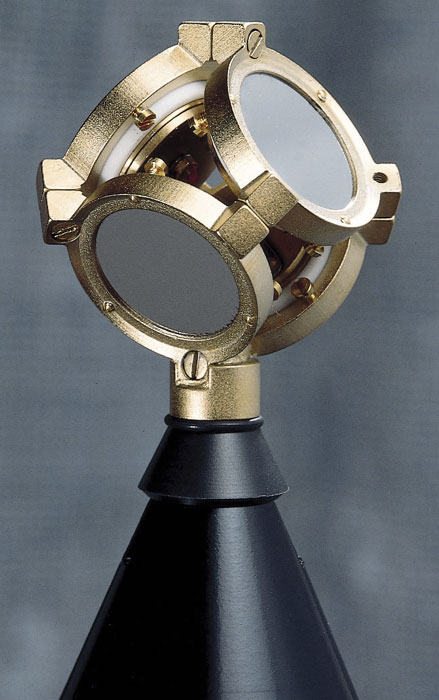
\includegraphics[scale = 0.2]{Sections/Background/images/soudFieldMic.jpg}
				\end{minipage}
				\begin{minipage}{0.5\textwidth}
					\center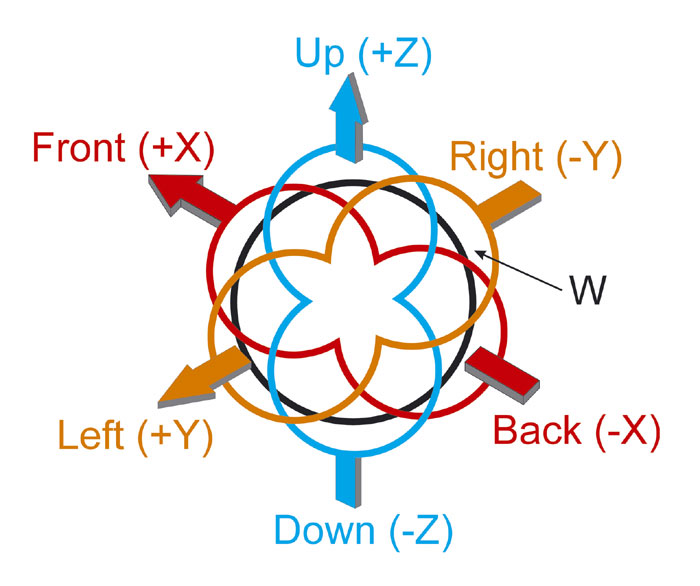
\includegraphics[scale = 0.3]{Sections/Background/images/soundFieldPolar.jpg}
				\end{minipage}
				\caption{\textbf{Left}: Picture of a Soundfield microphone with coincident capsules exposed \textbf{Right}: Soundfield microphone polar pattern \cite{soundFieldMic}}
				\label{sfMic}
			\end{figure}

		\subsection{Software Overview}

		\subsubsection{ODEON}
		\label{Software:Odeon}
		A method for measuring \ac{RIR}'s has been discussed, however there is also a way to synthesis \ac{RIR}'s by using room acoustic simulation software such as Odeon \cite{odeon}.

			Odeon was designed to provide reliable predictions of room acoustics by using a hybrid of two geometric acoustic models, Ray-tracing and the \ac{ISM} to synthesis \ac{RIR}'s. These methods model how sound would propagate around a room as though it were a straight line (ray). This inherently neglects wave phenomena such as phase and diffraction, properties that are negligible at high frequencies, however they are fundamental in describing low frequency wave behaviour \cite{Siltanen2010}. Therefore geometrical methods are not accurate at modelling sound propagation for low frequency waves.

			The reason for Odeon using a hybrid of the two method comes from the inherent problems encountered in each method.

		\paragraph{Ray-Tracing}
			The ray-tracing method imitates a sound source by emitting a large number of particles in various directions from a single point \cite{Rindel1995}. These particles are then traced around the room, losing energy each time the particle encounters a surface according to the absorption coefficient assigned to that surface. The angle at which the particle is then reflected is determined by the scattering coefficient assigned to the surface of contact, ranging from a specular reflection to a completely random reflection \cite{odeonManual}. For a specific receiver position, an area around said point is defined in which rays are collected and used to calculate the results.

			Ray-tracing does not provide a completely accurate result as it is a risk that some rays may not pass close enough to the receiver to contribute to the final result. The outcome of the ray-tracing method is a statistical result rather than a complete one.

		\paragraph{Image Source Method}

			%The \ac{ISM} represents specular reflections from surfaces as its own source, mirroring that of the original sound source, creating what is known as ``image sources'' \cite{Rindel1995} and can be used to find all possible specular reflection paths. Figure~\ref{ISMPic} illustrates this concept. The advantage of the \ac{ISM} is that each surface can be modelled by an image source which provides a great deal of data regarding the contribution to the received sound making this method more accurate than ray-tracing.

			The \ac{ISM} can be used to find all possible specular reflections paths from the sound source to the receiver position. This is done by representing each specular reflection from a surface as a secondary source known as an ``image source'' \cite{Rindel1995}, illustrated in figure~\ref{ISMPic}. The advantage of the \ac{ISM} is that each surface can be modelled by an image source which provides a great deal of data regarding the contribution to the received sound making this method more accurate than ray-tracing, however as each image source then emits more rays there is a possibility to produce a great deal more image sources. This means that the number of image sources grows exponentially for each new image source than is produced making this method much more computationally expensive than the ray-tracing method. This problem can be avoided by setting a \textit{reflection order} which determines how many times a ray can reflect off a surface before calculations are stopped, thus preventing the creation of more image source though the calculates for the prediction of the rooms acoustics will be incomplete. This obviously then makes the \ac{ISM} less accurate with a smaller reflection order.

			Once all image sources have been calculated, a visibility check is run. This checks to see whether the image sources that have been produced can be seen by the receiver, therefore checking whether that image source needs to be used or not. If the image source is not in sight of the receiver, it therefore does not need to be used for calculations. If the receiver position is moved, the visibility check is run again. Overall, this saves time as the image sources do not need to be recalculated.


			\begin{figure}[ht]
				\center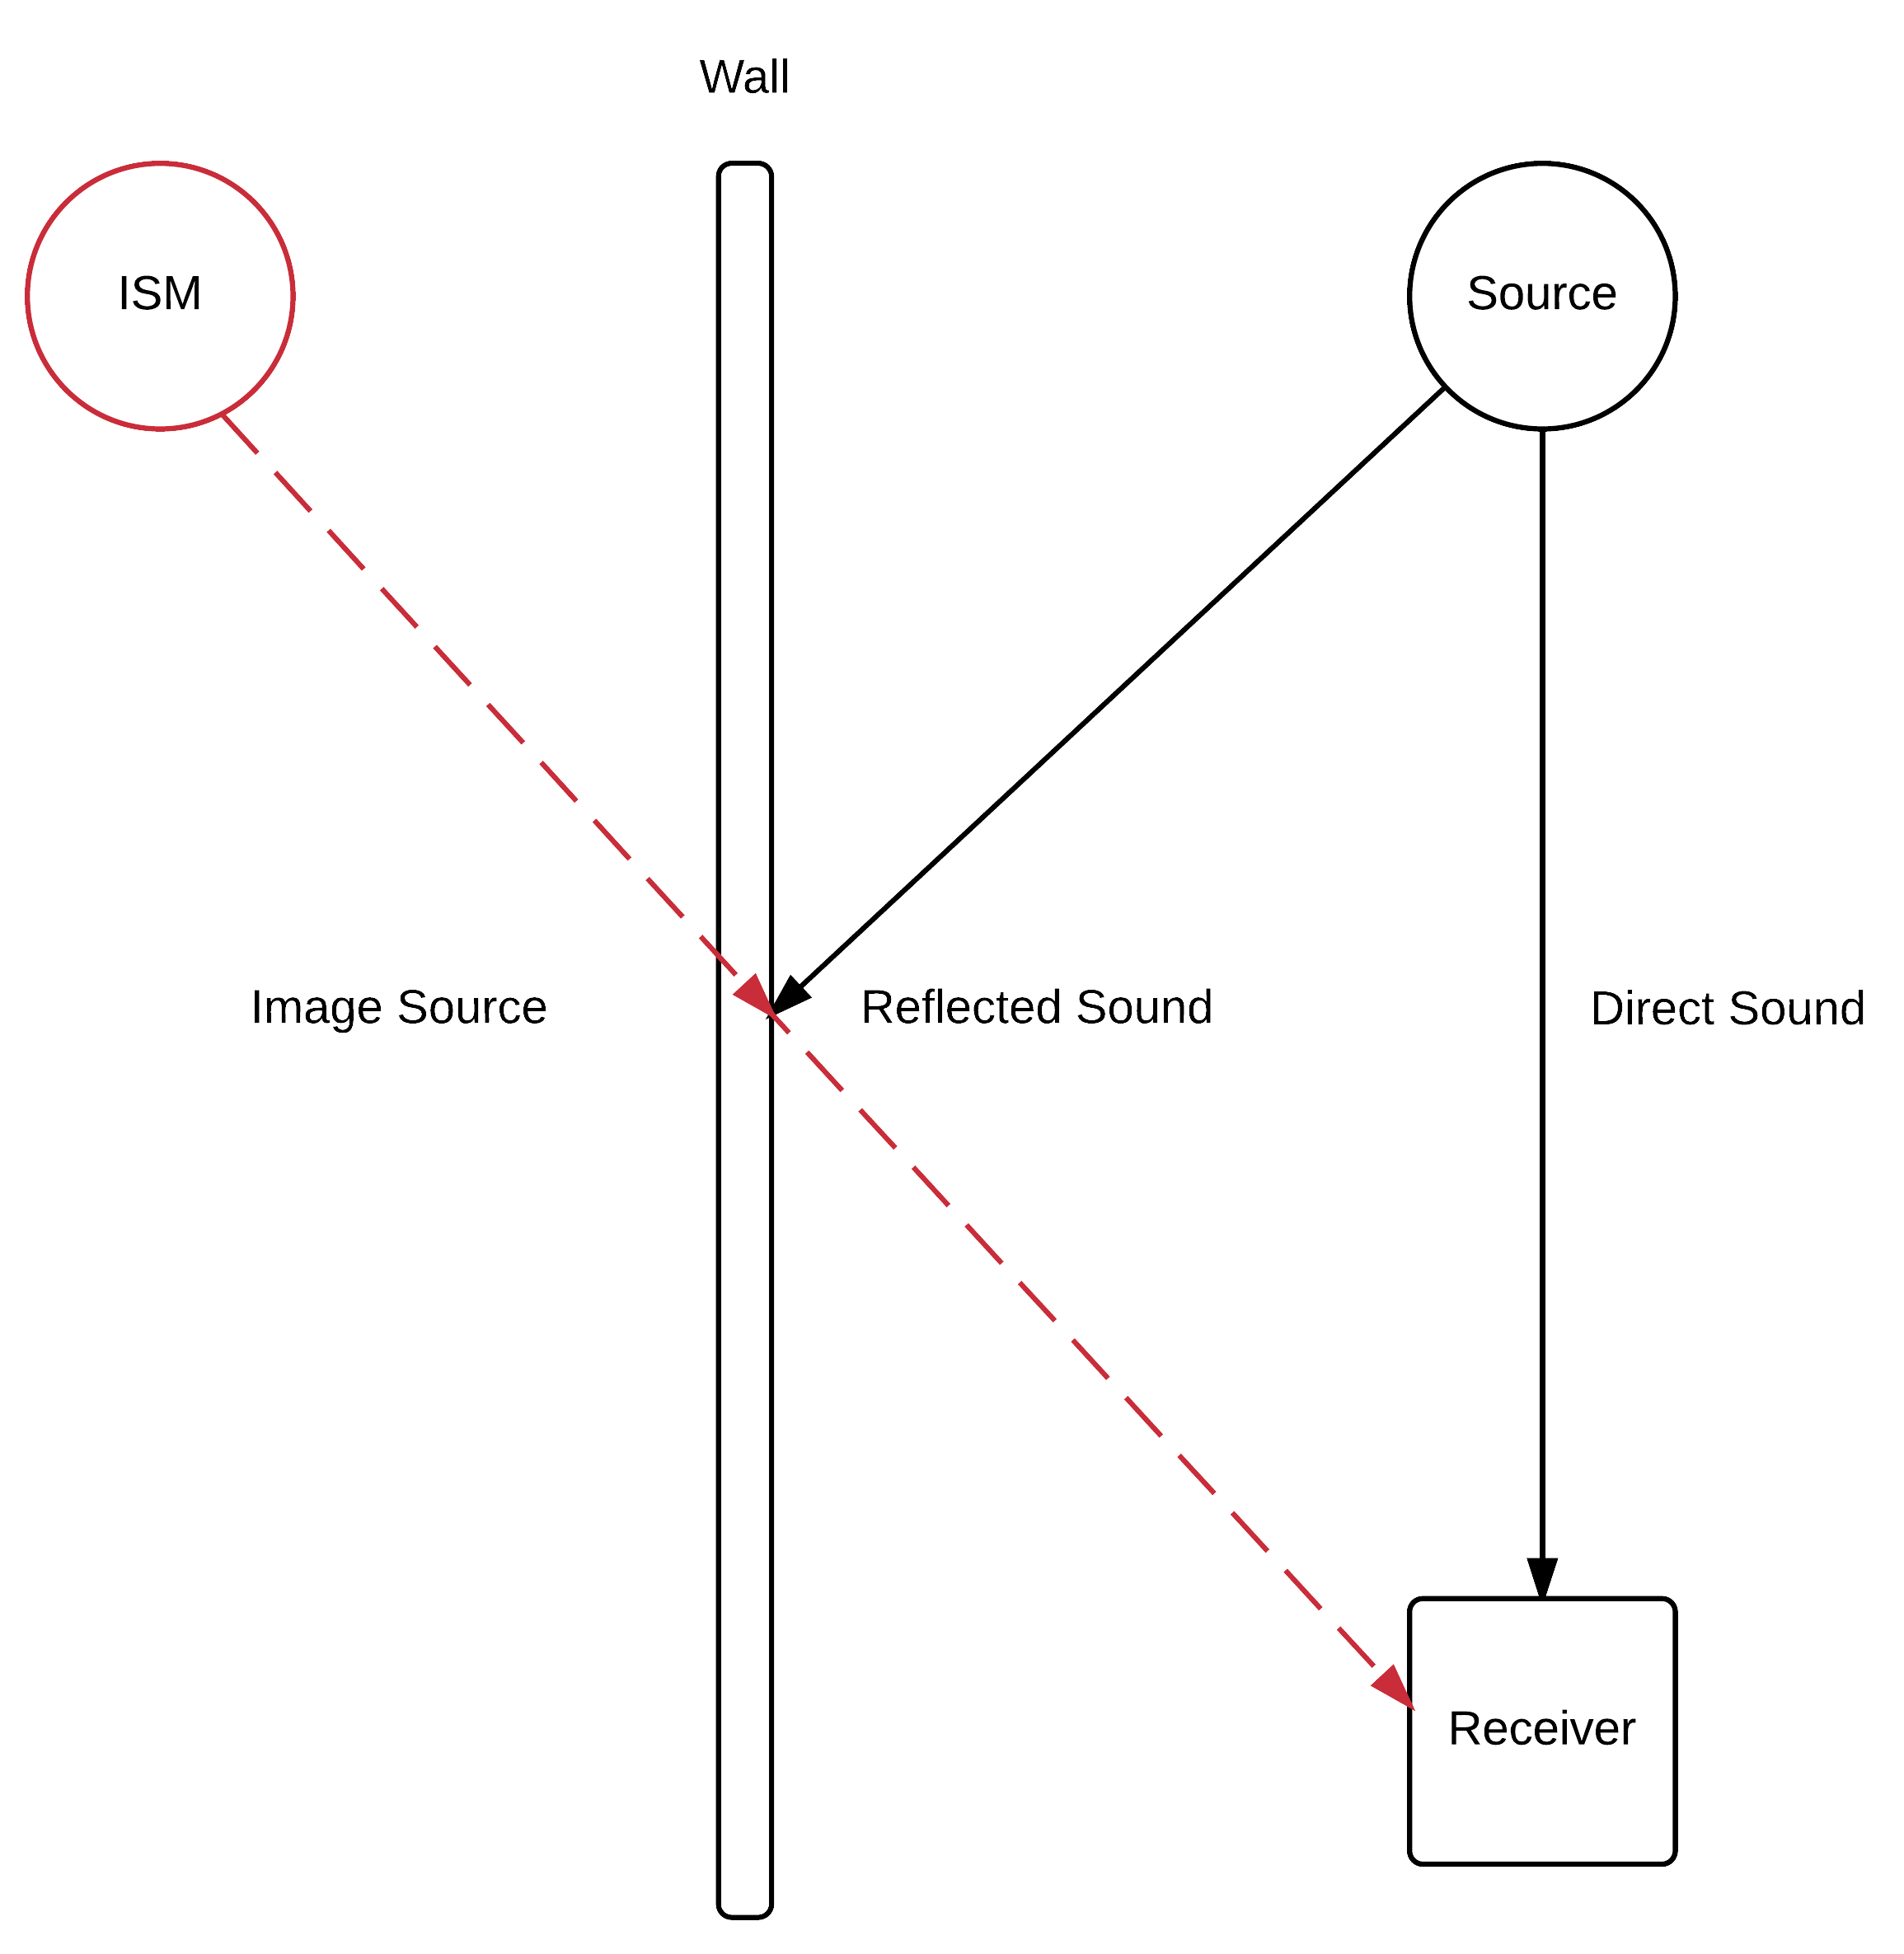
\includegraphics[scale = 0.3]{Sections/Background/images/ISM.png}
				\caption{Illustration of the image source method (by the author)}
				\label{ISMPic}
			\end{figure}

		\paragraph{Hybrid Method}
			%The inherent problems of the ray-tracing method and the \ac{ISM} are occluded by using a hybrid method that uses the best part of both. 

			Ideally, the \ac{ISM} would be used to calculate all sound rays due to its accurate results, however due to the computational limitations, Odeon uses a hybrid method to provide a reasonable compromise between calculation time and accuracy.

			The hybrid method first uses the \ac{ISM} to calculate a number of image sources up until a specified reflection order determined by a \ac{TO}. For example, if the \ac{TO} = 2, the image source method will allow a ray to reflect twice which will produce a number of image sources, then it will switch to using the ray tracing method to calculate a statistical model of how the rest of the rays might propagate. This gives the user the choice between computation time and accuracy.

		\paragraph{Scattering}
		\label{background:scattering}			
			Quote from Odeon Manual:	

			 \vspace{5mm}
		 \begin{center}
		 \begin{minipage}{0.5\textwidth}
		 \textit{``In short, each time ODEON detects an image source (IMS), an inner loop of (scatter) rays (not visualised in the 3D Investigate Rays display) is started, taking care of the scattered sound which is reflected from this image source /surface''}
		 \end{minipage}
		 \end{center}
		 \vspace{5mm}

		 \textbf{Reword that shit}

		\paragraph{Room Modelling}

			In order to predict the acoustics of a space, Odeon requires a geometry file in the form of a .par file. This file contains information regarding the room dimensions, object dimensions and positions. This can be produced within Odeon itself by using the built in `Extrusion Modeller' which allows a user to use a script like language to describe the rooms geometry. It is also possible to use 3rd party applications such as Google SketchUp \cite{SKU}, a software which is described in section~\fullref{GSU}.

		\paragraph{Material Selection}
			Selecting the appropriate absorption coefficients of the surfaces within a \ac{VAE} is crucial to its accuracy. Odeon provides a material list with common materials that can be assigned to the surfaces of a model read from a geometry file. This material list can be extended by creating new materials and assigning absorption coefficients to the appropriate frequency bands.

	\subsubsection{Google SketchUp}\label{GSU}
		Google SketchUp \cite{SKU} is an easy to use 3-D modelling software that can be used to produce room models. Unlike Odeon extrusion modeller, it allows the user the draw surfaces with a mouse, easily duplicate structures and provides simple measuring tools and markers to enable accurate modelling. Plug-ins such as SU2Odeon (``SketchUp to Odeon'') \cite{SU2Odeon} enables the user to convert the model into a .par file for Odeon to use as a geometry file.

	\subsubsection{Max/MSP}
		Max/MSP (Max) is a visual programming language that can be used to easily route and manipulate audio signals through the use of simple objects and patches \cite{max}. Max allows a number of external devices to be easily connected to the software such as smart phones and motion sensors through the use of plugins.

		\begin{center}
			\textbf{[More on Max]}
		\end{center}

		\paragraph{Spat}

			 Spat, developed at the research institute IRCAM \cite{spat} is designed for real-time spatialisation of sound signals in Max without having to touch any code. It provides an simple way to convolve B-format audio signals with impulse responses as well as decode the B-format signals for any given number of speakers in any arrangement by simply providing the number of speakers and angles at which they are placed.

\subsection{Project Description}
	\subsubsection{The Virtual Singing Studio}

		The \ac{VSS} is a loudspeaker based room acoustics simulator used as a tool for analysing the correlation between room acoustic characteristics and vocal performance parameters as part of Dr Jude Breretons PhD Thesis \cite{Brereton2014}. It is comprised of a head-mounted microphone used to capture a real-time audio input from a singer, a software patch that convolves the audio signal with a number of Ambisonic B-Format \ac{RIR}'s and finally a spherical array of 16 loudspeakers for which the convolved audio signal is decoded and fed to. In addition, a head-tracking device (an Oculus Rift \cite{oculus}) is also used to track which direction the user is facing in the virtual space. A flow diagram of the system can is shown in figure~\ref{vssDiagram}.

		\begin{center}
			\textbf{[Add VSS system diagram here]}
		\end{center}

		The \ac{VAE} used in the \ac{VSS} was initially the National Centre for Early Music, a space in York frequently used for musical performance. Using a Soundfield microphone, 16 Ambisonic B-Format \ac{RIR}'s were captured. Four positions were chosen and four \ac{RIR}'s facing in each direction (front, left, back, right) were recorded in each. These four directional \ac{RIR}'s are used to approximate the room acoustic phenomena that would occur if the user were projecting in that direction. This is done by using the data from the head-tracking device to amplitude pan the convolved signals before sending them to the spherical speaker array. Though this is a crude method for achieving such a state, it provides enough variation between the two directions to be considered convincing.


		\subsubsection{Project Motivation}
			
			%The \ac{VSS} has addressed a problem faced by professional musical performers: travelling to performance spaces for rehearsal.

			The \ac{VSS} addressed a problem faced when trying to research how musicians preform in different acoustic environments: having to travel to each performance space with musicians and researchers. This also indirectly provides a solution for performers wanting to rehearse is spaces that are often inaccessible and would otherwise be expensive to book and travel to. By obtaining an \ac{RIR} of the desired location, the only time travelling will be necessary is to initially obtain said \ac{RIR}. However, one limitation of using the \ac{VSS} is the restriction of position. If a performer wanted to try and sing at another point in the room, an \ac{RIR} would have to be taken in that position too. This could be done initially, taking a range of \ac{RIR}'s in a number of positions, however it cannot be guaranteed that all positions desirable to the performer will be available. Therefore, this project aims to implement a system that will allow the user of the \ac{VSS} to feel as though thy can move around a \ac{VAE} freely.

			%The initial implementation of the \ac{VSS} provided the user with a choice of four positions. To provide the user with more \ac{RIR} positions it could be possible to allow them to move where they choose.

			Previous projects have addressed mobility within \ac{VAE}'s before, such as \cite{Savioja1999}. The paper initially looks at two methods for providing mobility:

			%\textbf{direct} room impulse response rendering and \textbf{parametric} room impulse response rendering. Direct room impulse response rendering consists of obtaining a set number of \ac{RIR}'s in a grid and interpolation between them to synthesis the users position. This method suffered from the fact that a large number of \ac{RIR}'s are required, thus the requirement for a large amount of storage space.

			\begin{enumerate}

			 \item \textbf{Direct room impulse response rendering}: By producing a large grid of \ac{RIR}'s within the desired space, it is possible to allow a user to select a position in the room by interpolation between the two nearest neighbouring \ac{RIR}'s. This method does not provide truly accurate room acoustics for the selected location and also suffers from the fact that a large number of \ac{RIR}'s are required, thus the requirement for a large amount of storage space.

			\item \textbf{Parametric room impulse response rendering}: By actually synthesising \ac{RIR}'s in real time for the given position of the user in the \ac{VAE}, it is possible to provide an accurate \ac{RIR} for the given location. This method avoids the need for a large amount of storage space and a system to retrieve the correct files, however, as will be seen through the rest of this report, post-processing of the obtained {RIR}'s would not be possible with real time rendering.
			\end{enumerate}

			As the intention was to build upon the existing \ac{VSS} system, it was decided that the direct room impulse response rendering method would be used, as this method would allow for the modification of the existing patch used to real-time convolution.

			As the intention was to build upon the existing \ac{VSS} system which requires pre-recorded (and post-processed) \ac{RIR}'s, it was decided that the direct room impulse response rendering method was to be used and the effects of the issues related with the method studied.

			 %which would involve providing \ac{RIR}'s to the max patch to convolve with a real-time audio input, it was decided that the direct room impulse response rendering method was to be used and a way in which to provide the necessary \ac{RIR}'s was investigated. As mass storage is currently cheap and easily available, it was decided that the required number of \ac{RIR}'s to produce such as system was to be investigated, and whether the inaccuracy caused by interpolation between \ac{RIR}'s instead of producing location accurate \ac{RIR}'s is noticeable for the produced system.


		\subsubsection{Project Objectives}


			Given the aims of the project, the following questions are to be addressed:

			Given the project aims and the background provided, the following is a list of objectives that were set in order to complete this project:

			\begin{enumerate}
				\item Find an appropriate room to be modelled as a \ac{VAE} \\
				\item Digitally model the room using either Odeons extrusion modelling or 3rd part application \\
				\item Import room model into Odeon to finish material selection and \ac{RIR} settings\\
				\item Produce a grid of \ac{RIR}'s that can be used to interpolate between to simulate user positions\\
				\item Record real \ac{RIR}'s in locations that can be compared to synthetic \ac{RIR}'s\\
				\item Extend upon existing software patch to accommodate new functionality\\
				\item  Preform user tests:
					\begin{itemize}
						\item Does the perception of distance change when using real or synthetic \ac{RIR}'s?\\
						\item How far does the user have to move in the given \ac{VAE} before they notice they have moved \\
						\item How many \ac{RIR}'s are required for interpolation for the user to feel they are moving around the space freely\\
					\end{itemize}
				\end{enumerate}


	In order to test the perceptual differences when using synthetic RIRs, real RIRs of the same space had to be taken.

	Previous test in the VSS have required ‘Plausibility’ test, where the user must evaluate the response of the VSS without reference to the real venue. This is usually because testing a virtual environment against a real one (authenticity tests) requires travel which can be expensive and difficult. Therefore, by running test based on ‘plausibility’ a sense of how convincing the virtual room is can be obtained. In the case of other virtual reality systems where the virtual environment does not exist in the real world, only these types of test can be run.

	Though plausibility test are acceptable, an authenticity test gives more objective results. Therefore impulse responses of Hendrix Hall were taking, in the same format as the synthesised RIR’s.


		\subsubsection{Project Overview}

			The following outlines the steps that were required to produce a system that allowed a user to feel as though they are freely moving around a \ac{VAE} and the tasks necessary to investigate the plausibility of said system, thus completing the project aims and objectives set

		\subsubsection{Room Choice}

			The following room features were kept in mind when searching for a room to use as part of this project:

			\begin{center}
			\begin{tabular}{r p{12cm}}
				Size: & Large enough to be used as a singing space \\
				Simplicity: & Simple enough architecture to be able to model with the time available \\
				Accessibility: & The room had to be easily accessible to take  multiple measurements to make blue prints and take \ac{RIR} measurements
			\end{tabular}
			\end{center}

			The room chosen was Hendrix Hall, a large lecture theatre on the University of York campus. The room contains retractable seating leaving the large space in the centre open and unobstructed. The room is architecturally simple being almost perfectly rectangular with the occasional wall indent. With it being located on the universities campus it can be booked for any time of the week meaning it can be accessed when necessary and for free.



\end{document}